\chapter{Introduction}
\label{chap:intro}
Cloud computing, which utilizes a pool of computing resources to provision elastic, on-demand, and measured services via network, has reshaped the way that people use computers \cite{armbrust2010view}.  In the era of cloud computing, the centralized management of computational resources, such as data center, is not only more efficient, in terms of power and performance, to provide various services, but also supports higher security and availability to the provisioned services \cite{cully2008remus,gray1991high}.  One of the key technology to achieve those goals is virtualization \cite{goldberg1974survey, miller2007virtualization, yan2011development, singh2008server, chowdhury2010survey}. The abilities of virtualized machines to perform emulation, isolation, consolidation, and migration simply make resource management and high availability easier.

However, the service model of cloud computing is not perfect for all kinds of applications.  The recent advance of Internet Of Things (IOT) has brought new challenges that confront the centralized architecture of cloud computing.  A conservative estimation has shown that by the end of the decade, 22 billion connected devices will constantly generate semi-structured or unstructured data in real-time.  The interconnection of these devices will create immense data to strain the bandwidth and to lower the network availability. With such amount of network traffic, the centralized architecture will face huge amount of network failures or delays.  Moreover, many IOT services possess time sensitive data.  The network latency from the devices to cloud platforms can simply annihilate the possibility to fulfill the real-time requirement of IOT services.

One of the promising solutions is fog computing, proposed in {\color{red}\cite{bonomi2012fog,stolfo2012fog}}, which distributes massive number of decentralized edge nodes near IOT devices.  An edge node need not be as powerful as the cloud platform, but should be able to carry out a substantial amount of storage, communication, control, configuration, measurement and management of IOT devices.  Because of the proximity to end points, edge nodes can reduce the latency between devices.  In addition, the dense geographical distribution can help the quick recovery of failures with redundancy.

For an edge node in fog computing, virtual machines are no longer a good solution to deploy services, because of VMs' long booting time and large performance overhead.  An emerging technology, called container, appears just-in-time to fill the vacancy.  A container \cite{soltesz2007container} can be viewed as an operating system level virtual machine, which runs as an isolated process in userspace and shares the same kernel with other containers.  The kernel namespace \cite{biederman2006multiple} of host OS is used to isolate each container's environment, such as PID, IPC, network, and mount.  The cgroups in host OS can further control the hardware usage of each container, such as CPU, memory, network, and disk I/O.  Since containers need not to emulate the hardware, their performance is much better than that of Virtual Machine \cite{xavier2013performance, dua2014virtualization, joy2015performance}.  Figure \ref{fig:VM_vs_container} shows the architectural comparison between a virtual machine and a container.

\begin{figure}[h]
\begin{center}
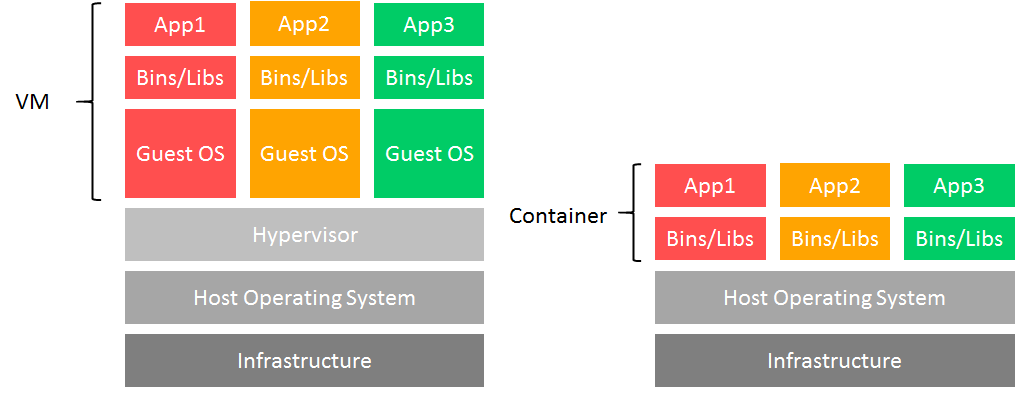
\includegraphics[width=15cm]{figure/VM_vs_container.png}
\end{center}
\caption{Virtual Machine and Container architecture}
\label{fig:VM_vs_container}
\end{figure}

Among many emerged container systems, such as LXC \cite{helsley2009lxc}, LXD, and Open VZ, Docker \cite{merkel2014docker} is the most popular container engine.  Docker uses Docker daemon to manage multiple containers in a single node.  Through the Command Line Interface (CLI), Docker clients can manage containers with operations, such as pulling a repository from the registry, running a container, committing a container to a new image, uploading the image to the registry, and terminating a running container.

On top of single containers, orchestration tools are essential to automate the deployment and operation of complex systems that involve multiple containers on cluster of edge nodes.  Several container orchestration tools have been or are being developed.  Kubernetes {\color{red} \cite{bernstein2014containers}} is a system developed by Google, which utilizes hierarchical architecture to manage thousands of containers for different systems on a large clusters. Apache Mesos {\color{red} \cite{hindman2011mesos}} is another orchestration system, whose original design is to co-allocate multiple heterogeneous distribute systems, such as MPI and MapReduce, into a group of machines.  Recently, it also includes containers into the system.

For fog computing, both Kubernets and Mesos may be too complex for a small cluster of edge nodes.  Alternatively, Docker Swarm {\color{red} \cite{DockerSwarm}}, which is a container orchestration system fully compatible with Docker commands, may be a better choice for managing containers on multiple edge nodes.

Docker Swarm is an on-going project with several under developing functions.  Our survey found that Swarm lacks of migration mechanism, which is critical for fail over and dynamic provisioning.  In addition, the current high availability support in Swarm is incomplete.  Swarm can only restart a failed container, but not resume its work.  Since for IOT fog computing, many real-time services may utilize in-memory methods to process data, restarting a failed container may loss many valuable data.

In this thesis, we propose a method that utilizes the checkpoint and restore mechanism to enhance the functionalities of current Docker Swarm implementation, migration and high availability more specifically.  Checkpoint and restoration \cite{Bhattiprolu:2008:VSC:1400097.1400109} can freeze a running process state and save the processing information to checkpoint images. Later, the checkpoint images can be restored to continue the process state.  Since a container is a special process in the host system, the checkpoint and restore is a right tool to use. In the design and implementation, we leveraged as many as Docker Swarm's APIs to make future integration easier.  We used Docker Swarm's scheduler to help the migration decision.  For high availability, we designed a multiple versions checkpoint mechanism to further enhance the availability.  Moreover, we investigated the methods to optimize the space and performance of checkpoint and restore.

{\color{red} We have designed 6 experiments, including the container migration performance and the influence of the parameters on container checkpoint time and container checkpoint image size.  The experimental results presents that the container checkpoint time will be affected by many ways, such as memory size and many container checkpoint at the same time, etc.  In addition, whenever we used pre-dump and track-memory technology, it will get better performance and use smaller storage in the most cases.}

{\color{red} The rest of this thesis is organized as follows.  Chapter \ref{chap:background} introduces the background of our thesis.  Chapter \ref{chap:design} presents implementation of system architecture,  Chapter \ref{chap:experiments} demonstrates the experimental results.  Chapter \ref{chap:related} presents related works.  Finally Chapter \ref{chap:conclusion} concludes the thesis. }